\chapter{Cambios en el método: uso de normales}
En las sección anterior nos encontramos con el siguiente problema: el método ICP funciona correctamente pero es demasiado lento ya que tiene un orden cuadrático y manejamos gran cantidad de información. Nuestro objetivo es entonces reducir el conjunto de puntos con los que trabajamos sin perder información. Este proceso no puede ser aleatorio y debe ser lo más significativo posible ya que, de lo contrario, podríamos obtener un resultado no deseado. Así usaremos en estos procedimientos los denominados \textit{descriptores}. Un descriptor lo podríamos definir como una medida de un punto en base a cierta característica que escojamos. De este modo obtenemos los llamados \textit{puntos significativos}, \textit{puntos clave} o \textit{key points} de cada una de las tomas. Como en nuestro marco de trabajo los modelos que tomamos como base son rígidos, es decir, no hay movimiento, cambios de escala, etc. podemos suponer que los puntos clave detectados en una toma deben de ser los mismos que en la otra. Por lo tanto, en una primera aproximación,  si realizamos el proceso para buscar la mejor transformación solo con los puntos clave deberíamos conseguir nuestro objetivo. \\

Como observación, aclarar que del mismo modo que no existe un método que funcione correctamente en el alineado de cualquier modelo, no existe un descriptor que funcione de manera adecuada con todos los modelos. Por ejemplo, podríamos detectar puntos clave en base al color. Si nos encontramos ante una escultura con un ropaje colorido y detallado es un descriptor que podríamos considerar válido. Sin embargo, si nuestro modelo presenta un color plano o una variación poco significativa del mismo no conseguiremos obtener puntos significativos. También debemos de tener en cuenta el tiempo necesario para la detección de puntos clave. El proceso debe ser lo suficientemente rápido para que reduzcamos el tiempo de alineación de las tomas y lo suficientemente bueno para que el conjunto de puntos calculado sea pequeño y descriptivo dentro de toda la nube.

\section{Variación de la normal}\label{varNormal}
El método para la obtención de puntos consistirá en la detección de zonas donde se produzca un cambio brusco de la normal calculando de este modo esquinas, hendiduras, etc.  Este procedimiento no es válido en superficies suaves ya que la variación de la normal en un entorno sería parecida en todo el modelo. Situación de este tipo nos la podemos encontrar, por ejemplo, en esferas. Una vez explicada la idea principal procedemos a explicar el proceso llevado a cabo. \\

En primer lugar, debemos calcular las normales de cada punto de la nube. Generalmente, es un proceso costoso aunque en nuestra  situación tenemos una gran ventaja. La información aportada por escáner con el que tomamos cada una de la muestras nos aporta, en cierta medida, una malla implícita ya que que puede entregar los datos de los puntos registrados siguiendo una cuadrícula en un archivo con formato PTX, que nos aporta el resultado por columnas por lo que podemos reconstruir la ``matriz'' espacial calculada previamente. Así con esta información para cada punto calculamos la normal mediante el producto vectorial de los triángulos adyacentes y luego promediamos obteniendo la de cada punto. En la figura \ref{Malla}, vemos a la izquierda la malla implícita que obtenemos con el formato que estamos trabajando. A la derecha aparece un ejemplo de cómo se han calculado las normales. En amarillo aparecen los vectores que se calculan (siempre y cuando existan dichos puntos) y en rojo los productos vectoriales necesarios. Destacamos que es importante que todas las normales tengan un convenio general de apuntar hacia dentro o hacia fuera del modelo. El nuestro ha sido de que apunten hacia afuera, lo que se ha tenido en cuenta durante la obtención de los productos vectoriales. \\

\begin{figure}[h!]
	
	\begin{minipage}{0.5\textwidth}
		\centering
		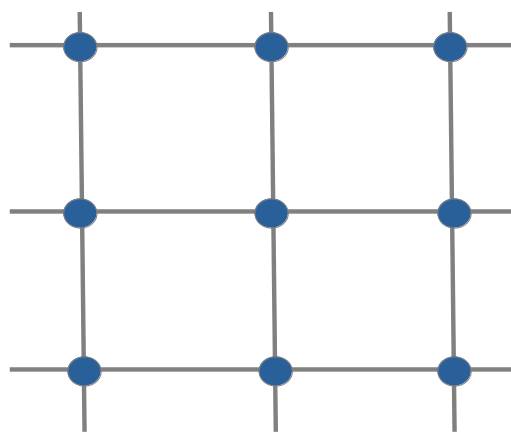
\includegraphics[width=0.65\linewidth, height=4cm]{Otros/Normal_1} 
		\caption*{(a)}
		%\label{fig:subim1}
	\end{minipage}
	\begin{minipage}{0.5\textwidth}
		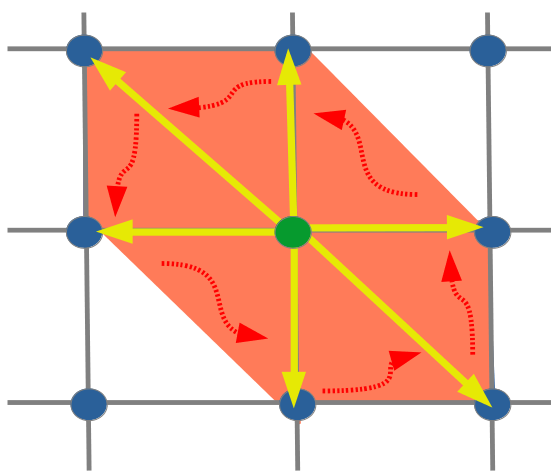
\includegraphics[width=0.8\linewidth, height=4cm]{Otros/Normal_2}
		\caption*{(b)}
		%\label{fig:subim2}
	\end{minipage}
	\caption{(a) Malla ímplicta, (b) Cálculo de la normal.}
	\label{Malla}
\end{figure}

La idea del algoritmo propuesto se basa en que en zonas relativamente planas las normales son muy parecidas por lo que la suma los productos escalares de la normal en un punto con aquellos contenidos en un entorno suyo es prácticamente 0. Razonemos lo que pasa en los lugares en los que hay esquinas. Tomamos un punto y sus vecinos, que en general son un total de 8. Suponemos una situación ideal en la que el punto que hemos escogido está en un borde. Si es así, consideramos que dos de los puntos adyacentes también están en dicho borde. \begin{comment}
INCLUIR DIBUJO !!!!!!!!!!!!!!!11
\end{comment} 
Así, tenemos que de sus vecinos adyacentes, dos tienen una normal parecida y los seis restantes perpendicular. Si calculamos el producto escalar medio en esta situación ideal obtenemos que es de $ 0.25 $. Por ello, el algoritmo propuesto tiene en cuenta este valor y solo se queda con los puntos cuyo descriptor de normales esté en un rango próximo al valor comentado, que pertenecería a la situación ideal. En nuestros experimentos hemos usado como criterio que el valor del producto escalar medio esté entre 0.15 y 0.3. \\

A continuación mostramos un ejemplo de los resultados obtenidos. Para ello, hemos usado diferentes niveles de precisión. Esto se ha conseguido simplificando la malla implícita que tenemos del modelo e indicando el número de filas y columnas que queremos conservar. Por ejemplo, si tenemos un nivel de precisión de 5, toma como puntos válidos aquellos que están cada 5 filas y 5 columnas. De este modo, de cada 25 puntos nos quedamos con uno. Si el nivel de precisión es 8, nos quedamos con un punto de 64. En la figura \ref{Ej_simpli} se muestran varios ejemplos de cómo varía la densidad de la malla en función del nivel de simplificado.
\begin{figure}[h!]
	\centering
	\begin{minipage}[b]{0.45\textwidth}
		\centering
		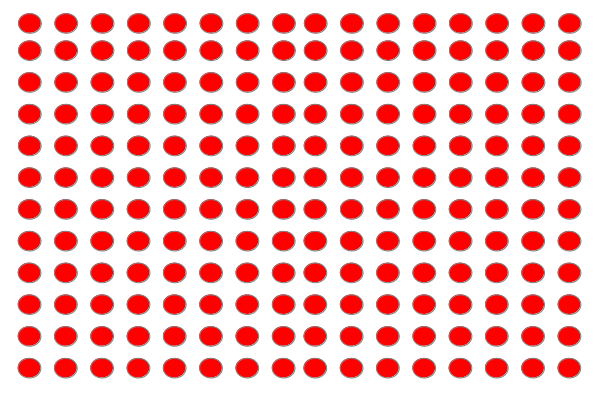
\includegraphics[width=0.7\textwidth]{Otros/Simp_0}
		\caption*{(a)}
	\end{minipage}
	\begin{minipage}[b]{0.45\textwidth}
		\centering
		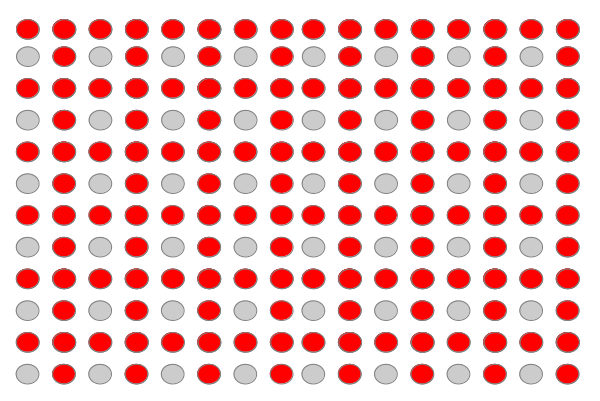
\includegraphics[width=0.7\textwidth]{Otros/Simp_2}
		\caption*{(b)}
	\end{minipage}
	\begin{minipage}[b]{0.45\textwidth}
		\centering
		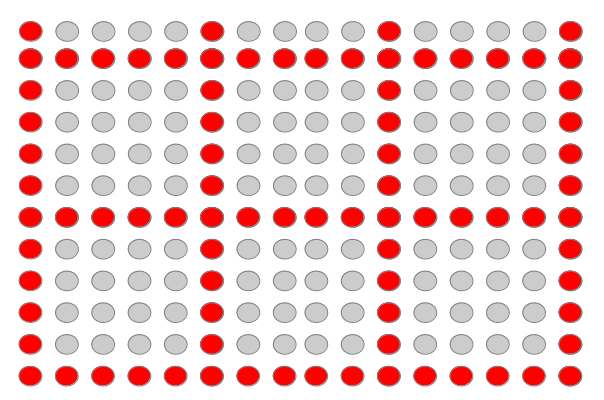
\includegraphics[width=0.7\textwidth]{Otros/Simp_5}
		\caption*{(c)}
	\end{minipage}
	\caption{Ejemplos de simplificado de la malla: (a) sin simplificado, (b) valor 2 y (c) valor 5. En rojo aparecen marcados los puntos con los que nos quedamos en cada caso.}
	\label{Ej_simpli}
\end{figure}

\begin{table}[h!]
	\centering
	\begin{tabular}{| c | c | c | c | c |} 
		\hline
		\thead{Nivel de\\ simplificado} & \thead{Puntos \\ totales}  & \thead{Tiempo cálculo \\normales (seg. )} & \thead{Tiempo cálculo \\ptos. clave (seg. )} & \thead{Puntos \\ clave} \\
		\hline
		1 & 2\,275\,886 & 25.1373 & 13.0592 & 592\,611 \\			 
		2 & 568\,830 & 6.39203  &  3.2690 & 192\,031 \\
		3 & 252\,881 & 2.82000 &  1.4716 & 46\,610 \\
		4 &  142\,186 &  1.72909 &  0.8370 & 11\,866\\
		5 & 90\,983 & 1.00018 & 0.5496 & 4490 \\
		8 & 35\,519 &   0.394472 &   0.2151 &  1\,885\\
		\hline
	\end{tabular}
	\caption{Resultados del cálculo de puntos clave. En la primera columna aparece el nivel de simplificado utilizado, en la segunda el número total de puntos de la malla (simplificada), en la tercera y cuarta se incluye el tiempo en segundos para el cálculo de las normales y el cálculo de los valores del descriptor respectivamente. En la última columna se aporta el número de puntos clave obtenidos en cada caso. }
	\label{table:desNormales}
\end{table}

\begin{figure}[h!]
	\begin{minipage}[b]{0.5\textwidth}
		\centering
		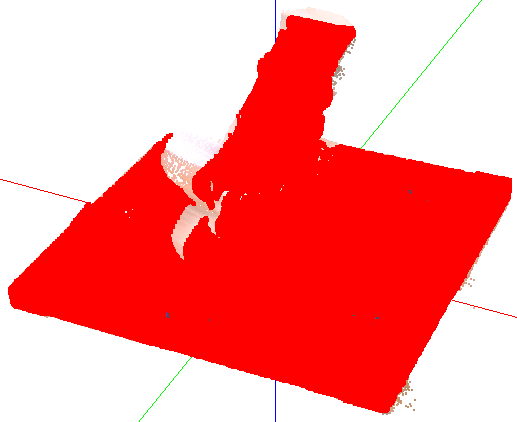
\includegraphics[width=0.7\textwidth]{ICP/desNormal-simp2}
		\caption*{Simplificado 2}
	\end{minipage}
	\begin{minipage}[b]{0.5\textwidth}
		\centering
		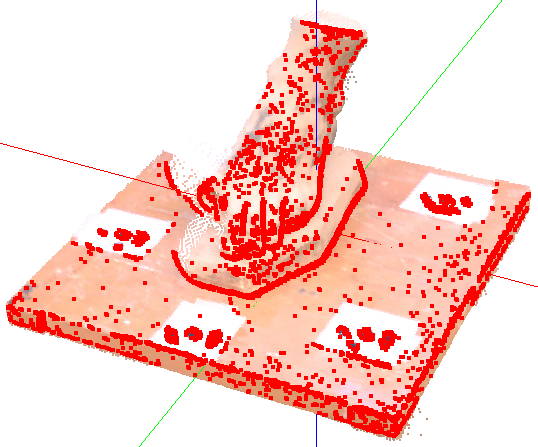
\includegraphics[width=0.7\textwidth]{ICP/desNormal-simp5}
		\caption*{Simplificado 5}
	\end{minipage}
	\begin{center}
		\begin{minipage}[b]{0.5\textwidth}
		\centering
		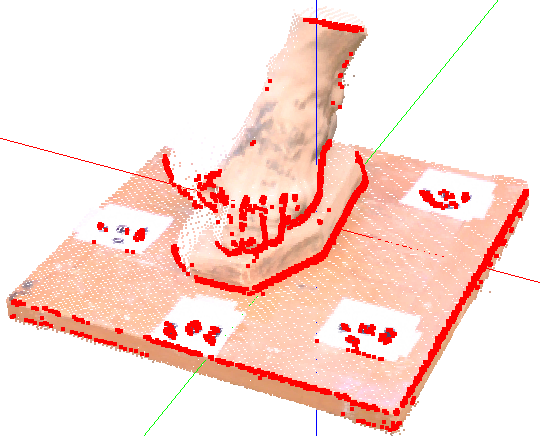
\includegraphics[width=0.7\textwidth]{ICP/desNormal-simp8}
		\caption*{Simplificado 8}
	\end{minipage}
	\end{center}
	\caption{Descriptor normales según el nivel de simplificado.}
	\label{Ej_simpli_real}
\end{figure}
Los resultados obtenidos tras aplicar el algoritmo de detección de puntos claves se muestran en la tabla \ref{table:desNormales} y figura \ref{Ej_simpli_real}. Vemos que uno de los problemas que tiene este método es que muy sensible al ruido. Esto, unido a la alta densidad de puntos con la que estamos trabajando hace que detectemos una gran cantidad de puntos clave. Por lo tanto, si queremos que los puntos obtenidos tras el proceso sean significativos tenemos que calcularlos a partir del modelo simplificado. Esto no debe de ser una problema ya que esto solo lo usaremos en las primeras iteraciones del método ICP ya que para obtener la solución deseada debemos tener en cuenta posteriormente el modelo entero debido a la sensibilidad del procedimiento. 

\section{Pruebas}
\subsection{De puntos clave a todo el modelo}
La primera prueba que se va a realizar es aplicar el procedimiento a los puntos clave pero tomados de parte de una toma a una otra toma completa que tomamos como modelo. Lo explicamos con nuestro ejemplo base del pie. Si probamos con las mismas tomas de la sección \ref{ejemPrac1} en las que solo aparece el pie los puntos que nos aportará el descriptor mediante normales es posible que no tengan una correspondencia clara con la otra toma, sobre todo, los que se encuentran en el borde. Por eso, debemos tomar como modelo la toma completa para asegurar en todo lo que posible que haya correspondencia entre los puntos clave aportados. Del mismo modo, también habría problemas si tomamos las dos tomas completas ya que nuevamente es probable que algunos puntos no estén en el modelo, y al intentar ajustarlos, nos aporte una solución errónea. \begin{comment}
Sección sola de aproximaciones erróneas
\end{comment} 
Destacamos que aplicar el procedimiento propuesto a una parte de las tomas no debe de ser restrictivo porque nos interesa conocer la transformación. Podríamos almacenar los datos de las transformaciones que se van realizando y posteriormente aplicarlo a la toma completa. Otra solución sería, por ejemplo, imponer una distancia máxima entre dos puntos para asegurarse de que realmente se corresponden. Esta solución será la que usaremos en la siguiente sección.\\

\begin{figure}[h!]

	\begin{minipage}[b]{0.5\textwidth}
		\centering
		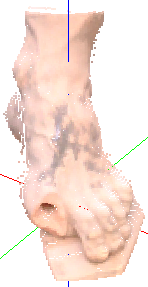
\includegraphics[width=0.3\linewidth]{ICP/prueba_ICP_3_1} 
		\caption*{Conjunto (1) con  7\,527 puntos.}
		%\label{fig:subim1}
	\end{minipage}
	\begin{minipage}[b]{0.5\textwidth}
		\centering
		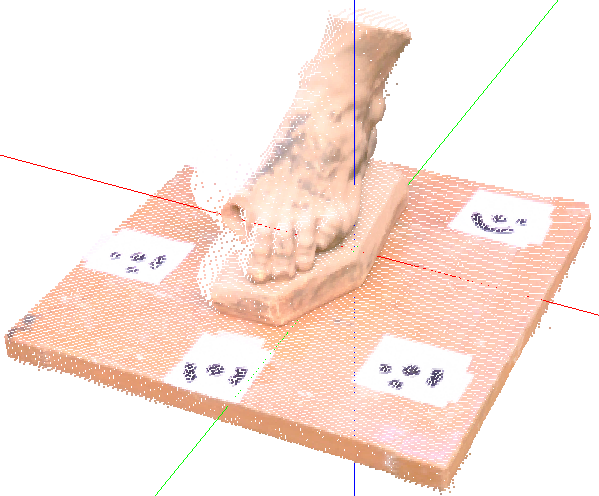
\includegraphics[width=0.6\linewidth]{ICP/prueba_ICP_3_2}
		\caption*{Conjunto (2) con 79\,921 puntos.}
		%\label{fig:subim2}
	\end{minipage}
	
	\caption{Tomas a alinear.}
\end{figure}

El número de puntos característicos detectados en la toma de la izquierda mediante el descriptor de las normales en el intervalo (0.15, 0.3) es de 506. Aplicamos el procedimiento y los resultados obtenidos se muestran en la figura \ref{clave1} y en la tabla \ref{table:ICPKPtotal}.\\

\begin{figure}[h!]
	\begin{minipage}[b]{0.5\textwidth}
		\centering
		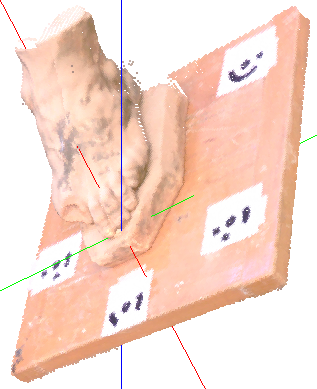
\includegraphics[width=0.65\linewidth]{ICP/prueba_ICP_3_3} 
		\caption*{Situación inicial.}
		%\label{fig:subim1}
	\end{minipage}
	\begin{minipage}[b]{0.5\textwidth}
		\centering
		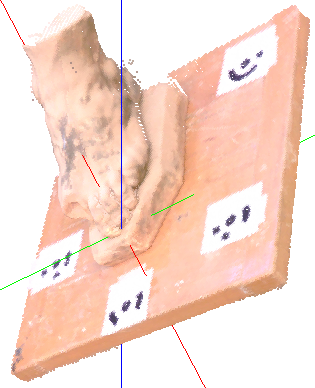
\includegraphics[width=0.65\linewidth]{ICP/prueba_ICP_3_4}
		\caption*{Resultado tras una iteración.}
		%\label{fig:subim2}
	\end{minipage}
	\begin{center}
		\begin{minipage}[b]{0.5\textwidth}
		\centering
		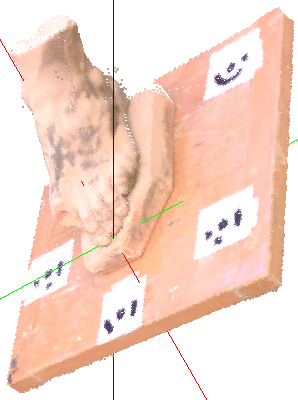
\includegraphics[width=0.65\linewidth]{ICP/prueba_ICP_3_5}
		\caption*{Resultado final.}
		%\label{fig:subim2}
	\end{minipage}
	\end{center}

	\caption{Algoritmo ICP usando un conjunto de puntos clave.}
	\label{clave1}
\end{figure}

\begin{table}[h!]
	\centering
	\begin{tabular}{| c | c | c | c |} 
		\hline
		Iteración & Dist. antes (mm)  & Dist. después (mm) & Segundos \\
		\hline
		1 &  23.3617 &  16.9620 & 20.0778\\			 
		2 & 16.1331 & 15.4993 &   19.7434\\	
		3 & 15.2290 & 15.0944  & 19.4636\\
		4 & 14.9740 &  14.9382 & 19.4807\\
		\hline
	\end{tabular}
	\caption{Resultados ajuste mediante ICP.}
	\label{table:ICPKPtotal}
\end{table}

Vemos que el procedimiento funciona correctamente y además que el tiempo empleado se reduce considerablemente respecto a los tiempos que habríamos necesitado considerando los conjuntos completos. Para hacernos una idea de ese tiempo basta tomar el ejemplo del pie de la sección \ref{ejemPrac1}. En ese caso, los conjuntos tenían unos 7\,000 y 8\,000 puntos cada uno y tardaba poco más de un minuto. Ahora unos de ellos tiene casi 80\,000, por lo que teniendo en cuenta el orden cuadrático del método, incrementaría bastante el tiempo necesario para completar cada iteración. Destacar que al igual que el procedimiento original, es posible que el resultado obtenido no sea el deseado y tenga que aplicarse desde el principio.
\subsection{De puntos clave a puntos clave}
Nuestro propósito ahora es intentar reducir aún más el conjunto de puntos con los que realizar el proceso ICP. Para ello, vamos a probar qué pasa si aplicamos el algoritmo solamente a los conjuntos de puntos clave calculados. Este paso hay que hacerlo con cuidado ya que, incluso en mayor medida que tomando en una muestra la toma entera, nos arriesgamos a que muchos puntos no tengan una correspondencia. Así, para el cálculo del punto más cercano se ha tenido en cuenta: 

\begin{enumerate}
\item Solo se comprueban puntos clave con un valor de descriptor parecido. Así, se ha fijado una diferencia máxima permitida y solo se comprueban los puntos que tengan un valor dentro de ese intervalo. Este se debe a que al ser movimientos rígidos no hay ningún tipo de deformación por lo que los planos serán los ``mismos'' mismos entre una toma y otra. Sin embargo, ponemos un intervalo debido a los errores del escáner y a las pérdidas de precisión debido al simplificado del modelo para la obtención de puntos clave.
\item Se ha acotado la distancia máxima permitida para un punto. Así, una vez calculada la distancia mínima de un punto al otro conjunto comprobamos que esa distancia no supere un umbral que hemos prefijado. Si lo supera significa que el punto más cercano está demasiado lejos y por ello no se corresponden realmente. De este modo, nos aseguramos que zonas que no se solapen se intenten ajustar y acabemos teniendo una solución errónea. 
\end{enumerate}

En la figura \ref{fig:KPKPICP} mostramos un ejemplo del resultado obtenido imponiendo que los valores de los descriptores entre los puntos claven difieran en $ 0.01 $ y que la distancia (en metros al cuadrado) entre ellos no sea mayor a $ 0.1 $. \\

\begin{figure}[h!]
	
	\begin{minipage}[b]{0.5\textwidth}
		\centering
		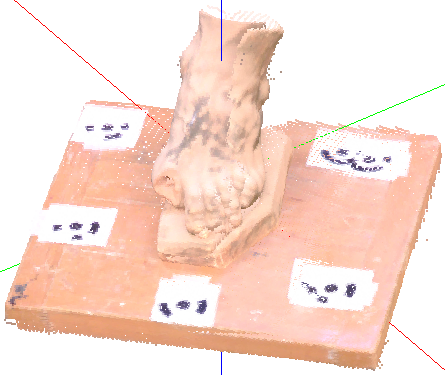
\includegraphics[width=0.9\linewidth]{ICP/prueba_ICP_4_1} 
		\caption*{Tras prealineado.}
		%\label{fig:subim1}
	\end{minipage}
	\begin{minipage}[b]{0.5\textwidth}
		\centering
		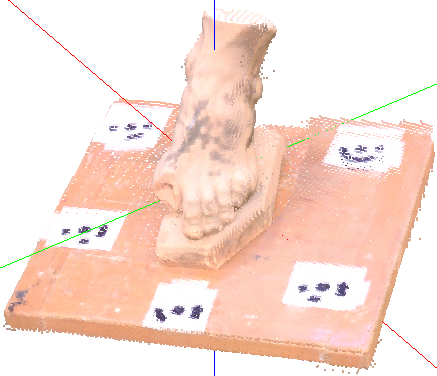
\includegraphics[width=0.9\linewidth]{ICP/prueba_ICP_4_2}
		\caption*{Tras dos iteraciones.}
		%\label{fig:subim2}
	\end{minipage}
	\caption{Proceso ICP solo con puntos clave.}
	\label{fig:KPKPICP}
\end{figure}

Se han realizado dos iteraciones. En ambas ha tardado aproximadamente 0.7 segundos y la distancia media (en milímetros) ha variado de 27.9743 a 26.8752. Los puntos clave calculados en cada caso son en el primera toma un total de $ 1\,142 $ y en la segunda $ 2\,273 $. Observamos cómo tras las dos iteraciones se han conseguido ajustar mejor las dos tomas. Nuevamente, hacemos hincapié en que el algoritmo ha tardado menos de lo que habría necesitado en caso de haber tomado las nubes de puntos completas gracias a la reducción del número de elementos de ambos conjuntos. \\

Una segunda aproximación es contar el número de productos escalares que dan ``cero'' para saber el número de planos perpendiculares que tiene cada punto. De este modo, solo comparamos con puntos cuyo número de ceros es el mismo. Se ha tomado perpendicularidad cuando el producto escalar sea menor que 0.01 debido a errores en la toma de muestras y simplificado de la malla. Notar que seguimos teniendo en cuenta la cota de la distancia máxima. Esto puede hacer que en un paso del método la distancia puede ser mayor que el anterior al existir un mayor o menor número de puntos que se han tomado como referencia. Esto no debería ser ningún problema \textit{a priori}. En el ejemplo que hemos usado ese número no ha variado entre iteraciones. En la tabla \ref{talbe:ICPceros} se recogen los resultados para cada iteración.\\

\begin{table}[h!]
	\centering
	\begin{tabular}{| c | c | c | c |} 
		\hline
		Iteración & Dist. antes (mm)  & Dist. después (mm) & Segundos \\
		\hline
		1 &  35.2816 &  34.8378 & 2.33132\\			 
		2 & 34.6116 &  34.4906 &   2.32062\\	
		3 &  34.4138 & 34.3591  & 2.30985\\
		4 & 34.3277 &  34.3057 & 2.32283\\
		\hline
	\end{tabular}
	\caption{Resultados ajuste mediante ICP del modelo del con puntos clave agrupándolos por el número de ceros de sus productos escalares.}
	\label{talbe:ICPceros}
\end{table}

\begin{figure}[th!]
	
	\begin{minipage}[b]{0.5\textwidth}
		\centering
		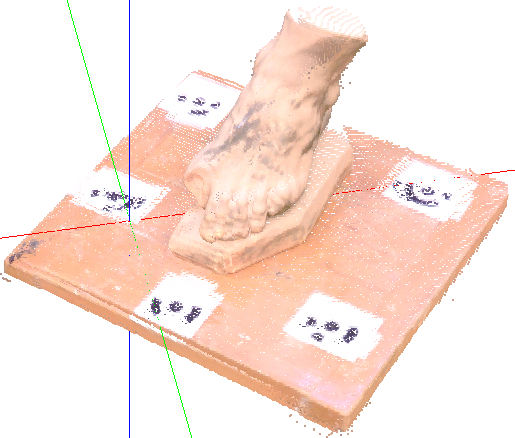
\includegraphics[width=0.9\linewidth]{ICP/prueba_ICP_5_1} 
		\caption*{Tras prealineado.}
		%\label{fig:subim1}
	\end{minipage}
	\begin{minipage}[b]{0.5\textwidth}
		\centering
		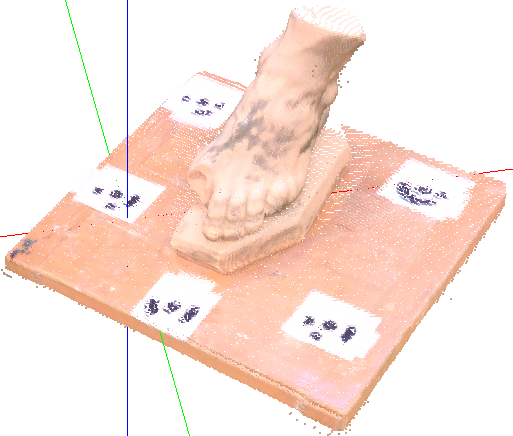
\includegraphics[width=0.95\linewidth]{ICP/prueba_ICP_5_2}
		\caption*{Tras cuatro iteraciones.}
		
		%\label{fig:subim2}
	\end{minipage}
	
	\caption{Proceso ICP solo con puntos clave agrupándolos por el número de ceros de sus productos escalares.}
	\label{fig:ICPej5}
\end{figure}

Con este procedimiento, en la figura \ref{fig:ICPej5} vemos que nuevamente se ha obtenido un proceso satisfactorio en la zona de los dedos del pie aunque ha tardado más tiempo en cada iteración que en el caso anterior.